\section{Глава 4}
\label{ss:hw}

Задачей полунатурного эксперимента являлась верификации возможности применения предлагаемого подхода к оценке параметров сигнала СПИ с ШПС. Для определения наличия источников
сигнала был применен классический параллельный коррелятор \cite{tsui} с шагом по частоте 1 кГц и диапазоном 5 кГц. Данный диапазон обусловлен максимальным Допплеровским
смещением частоты для стационарного приемника в СПИ Navstar GPS \cite{shahtarin_sync, tsui}. 

\subsection{Аппаратная платформа}
Представленная аппаратная платформа была разработана автором в процессе дипломного проектирования в Московском Государственном Университете Приборостроения и Информатики (МГУПИ).

Данная аппаратная платформа предоставляет пользователю возможность получать необработанный сигнал со спутников СНС Navstar GNSS. В текущей реализации поддерживается только 
СНС Navstar GPS, однако чип так же может принимать сигналы СНС Galileo и СНС Глонасс. Дампы данных представляют собой текстовые файлы. В них содержится 256 КБ необработанных данных.
На частоте оцифровки 256 КБ представляет чуть более 6 мс данных. Данного объема хватает для оценки параметров источников сигналов СНС Navstar GPS.
В данный момент аппаратная платформа используется как лабораторный стенд в МГУПИ по курсу ЦОС. Платформа позволяет работать с реальным сигналом, что является большим плюсом в
виду того, что позволяет наглядно продемонстрировать работу алгоритмов обработки сигнала, а так же проверить теоретические предположения в реальных условиях.
Так же на базе платы разрабатывается ряд дипломных работ в области СНС систем (например создание аппаратного коррелятора на VHDL или создание модели канала 
СПИ Navstar GPS данных). Исходники прошивки платы расположены в публично доступном хранилище кода github.com \cite{github-gpsproject}.
Там же опубликована разводка платы в формате программы PCAD и BOM (bill of materials).

Компонентами на плате управляет FPGA-микросхема. В ней содержится контроллер памяти, реализация RS-232 интерфейса, последовательный интерфейс программирования микросхемы
MAX2769 компании Maxim Semiconducter, модуль захвата данных, а так же вспомогательные модули. В рабочем режиме плата ждет команд с RS-232 интерфейса.
Команды выдает управляющее ПО (board daemon) - сервис разработанный под ОС GNU Linux.

Схема аппаратного обеспечения, настроенного на двухквадратурный прием сигнала СНС Navstar GPS с двухбитным режимом работы АЦП, приведена на рисунке \ref{pic:board_scheme}.
\begin{figure}[H]
	\center\scalebox{1}{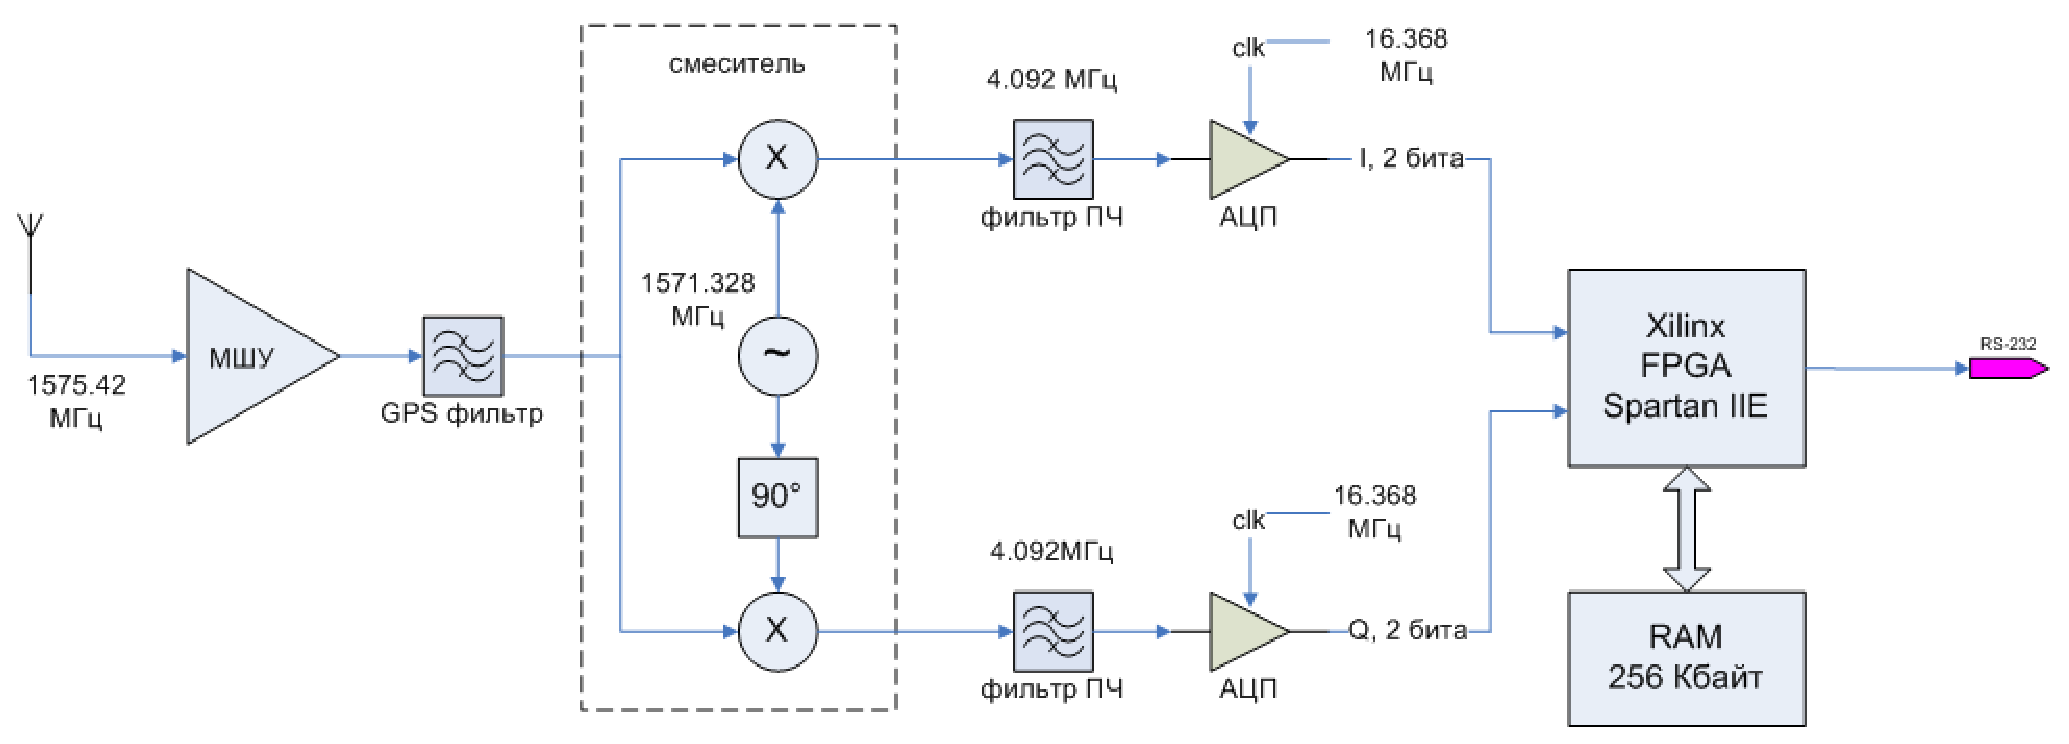
\includegraphics[width=1\linewidth]{board_scheme.eps}}
	\caption{Схема аппаратного обеспечения}
	\label{pic:board_scheme}
\end{figure}

Схема системы по захвату данных представлена на рисунке \ref{pic:gps_acq_system_scheme}. Данная система работает по схеме отложенной обработки данных. Основной сервер системы захвата
выдает команду оборудованию захвата - начать накопление данных. Оборудование захвата данных переходит в режим захвата и начинает накапливание 256 КБ данных. По окончании цикла
накопления данных оборудование захвата данных отвечает о готовности данных основному серверу системы захвата и начинает передачу данных. После передачи данных основной сервер
захвата данных публикует на публичный FTP-сервер файл с данными и прилагает к нему WAAS-картинку, которая отображает положения спутников над землей. Файл с данными
и картинку WAAS может забрать с FTP-сервера клиент для последующей работы с данными на своем ПК. В качестве диплома автор также разработал SDK для работы с файлом данных
\cite{github-gpsproject}: функции загрузки данных в MATLAB, параллельный коррелятор, генератор ПСП Голда и некоторые другие функции для облегчения работы с аппаратной платформой
и данными.

\begin{figure}[H]
	\center\scalebox{1}{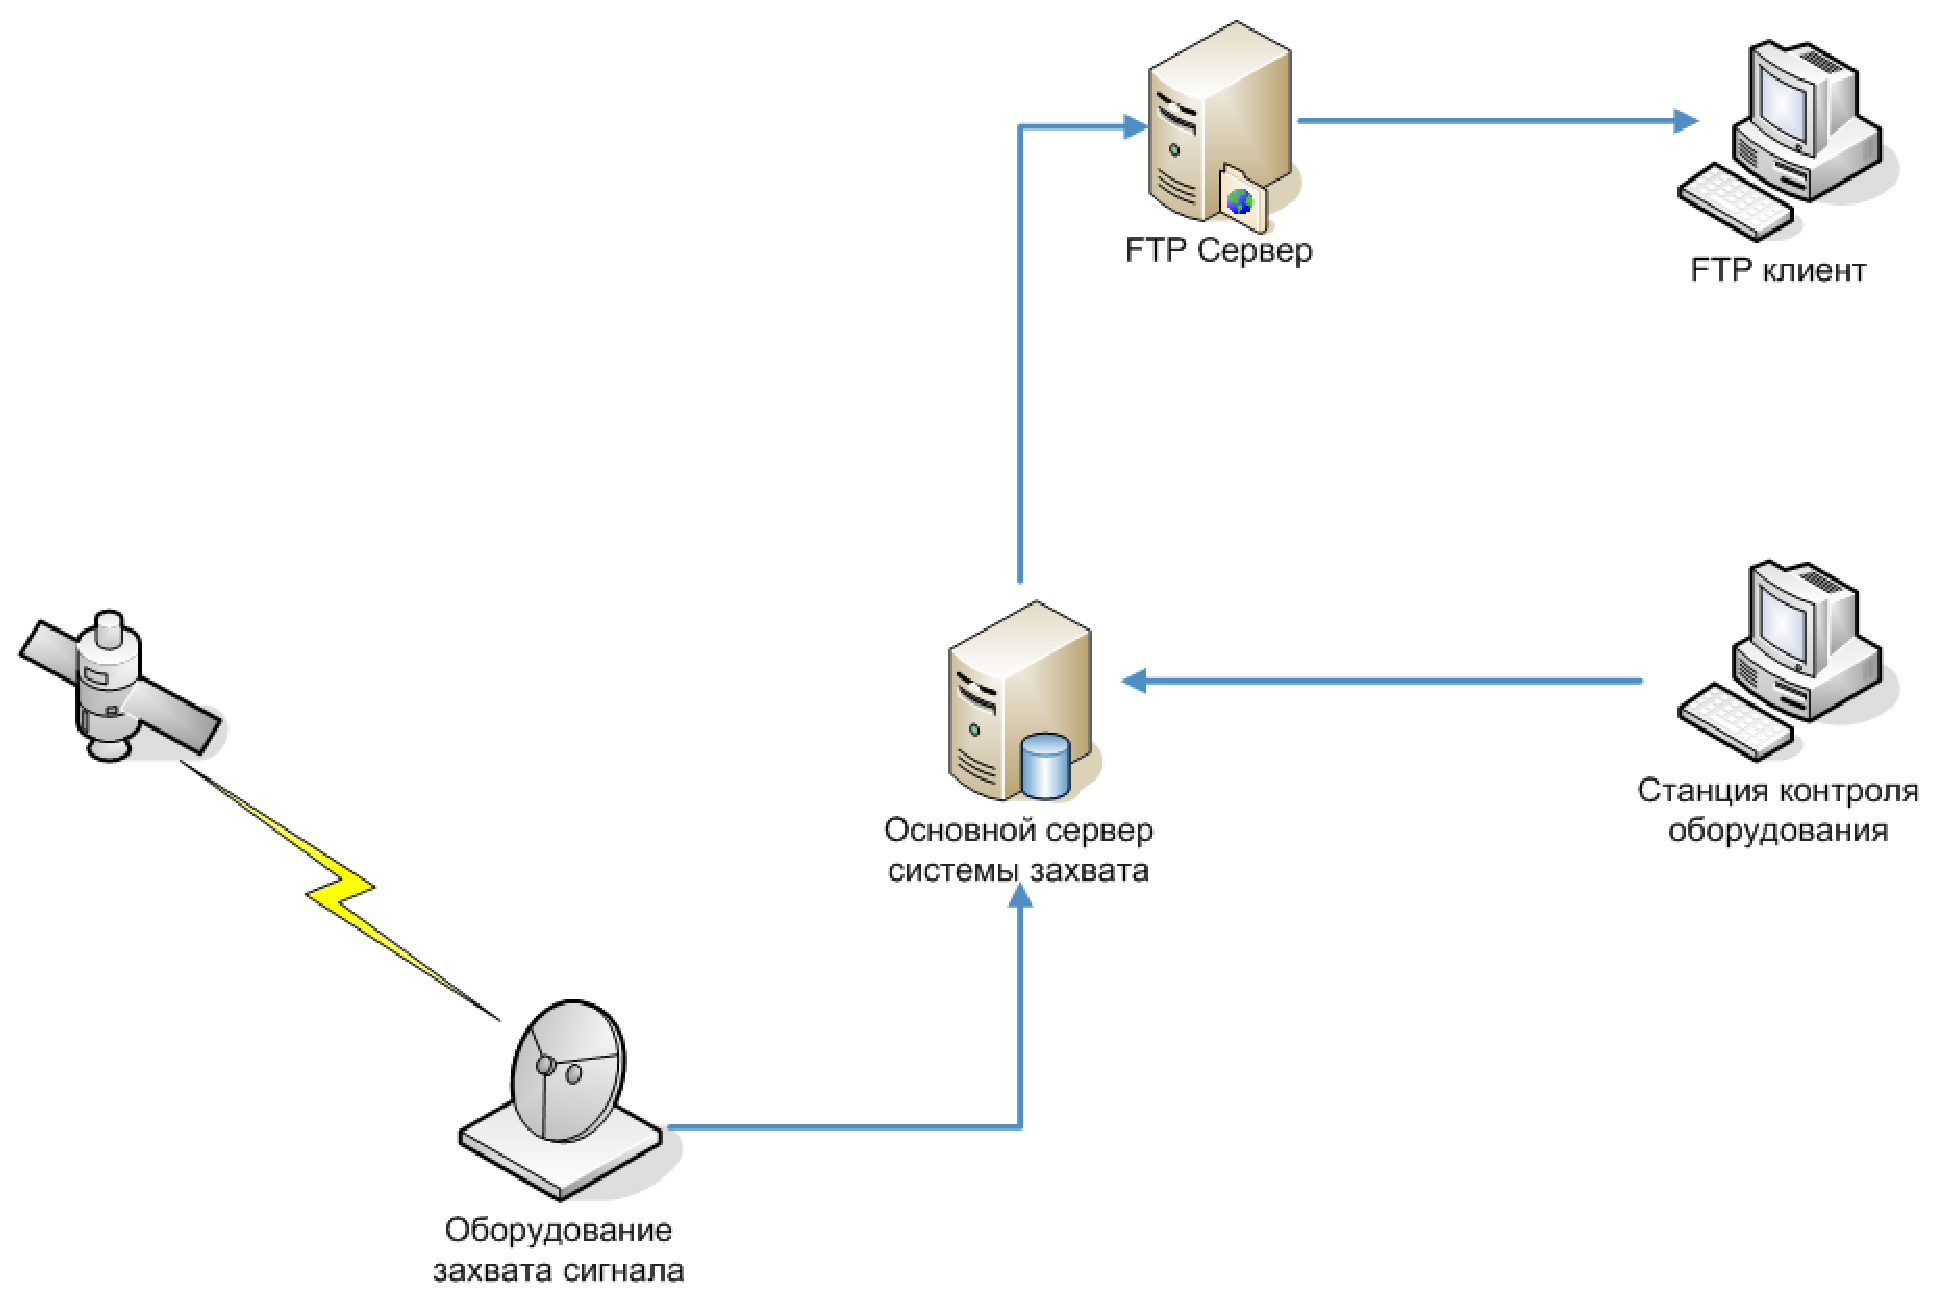
\includegraphics[width=1\linewidth]{gps_acq_system_scheme.eps}}
	\caption{Схема системы захвата данных}
	\label{pic:gps_acq_system_scheme}
\end{figure}

Структура файла с данными представлена на рисунке \ref{pic:dump_file}. В файл записываются значения управляющих регистров микросхемы MAX2769 для того, чтобы можно было
понять в каком режиме был записан файл. К доступным режимам, например, можно отнести \cite{max2769_manual}: одно- или двухквадратурный режим работы, разрядность при оцифровке
аналогового сигнала, тип захватываемых данных СНС (Глонасс, Navstar GPS, Galileo), а так же другие.

\begin{figure}[H]
	\center\scalebox{0.5}{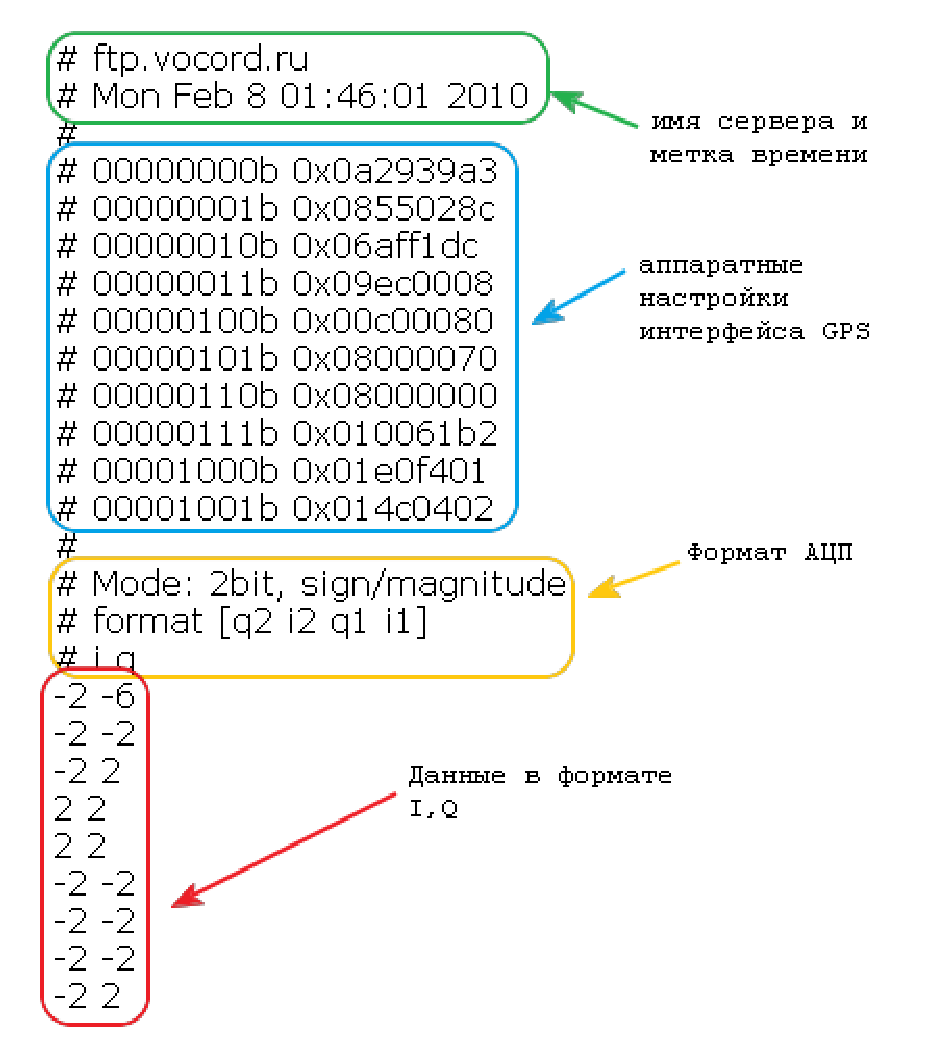
\includegraphics[width=1\linewidth]{dump_file.eps}}
	\caption{Структура файла с данными}
	\label{pic:dump_file}
\end{figure}

\subsubsection{Результаты эксперимента}

\subsection{Эксперимент на данных Мишеля Боваро}

Так же полунатурное моделирование проводилось с данными собранными итальянским ученым Мишелем Боваро (Michele Bavaro) \cite{bovaro_blog}. Представленный файл с данными оцифрован
с частотой 5.456 МГц, промежуточная частота источников сигнала, 4.092 МГц. Длинна записанных данных позволяет так же проверить
вхождение системы в синхронизм. Файл больше недоступен по ссылке, приведенной в блоге Мишеля Боваро, автор представляет его по адресу \cite{rflab_primo}.
В качестве алгоритма оценки фазы ПСП использовался
рассмотренный алгоритм DMA, оценка частоты проводилась при помощи алгоритма основанного на применении авторегрессионной модели (АР), предложенной авторами в \cite{FIXME-otchet}.
Полученная оценка подавалась на модуль фазовой автоподстройки частоты (ФАПЧ) и проверялось вхождение в синхронизм.

Для увеличения ОСШ в алгоритме DMA использовалось когерентное накопление сигнала. Производилось осреднение на 3 мс сигнала, что дает прирост ОСШ на 4.77 дБ.
В алгоритме на основе АР метода была взята 1 мс сигнала дополненная 3 мс нулей, для повышения спектрального разрешения при оценке АКФ посредством ДПФ.

В качестве модуля ФАПЧ взят код американского ученого Дениса Акоса (Dennis M. Akos) \cite{sandiaproject}.
Параметры выбранные для ФАПЧ: коэффициент демпфирования ${\zeta=0.7}$, шумовая полоса  ${B_L=40}$ Гц. 

\subsubsection{Результаты эксперимента}

Результат работы классического коррелятора представлен на рисунке \ref{pic:5mhz_sats_all}. Сигнал взят с 2000 отсчета, данное смещение выбрано произвольно.
\begin{figure}[H]
\center\scalebox{1}{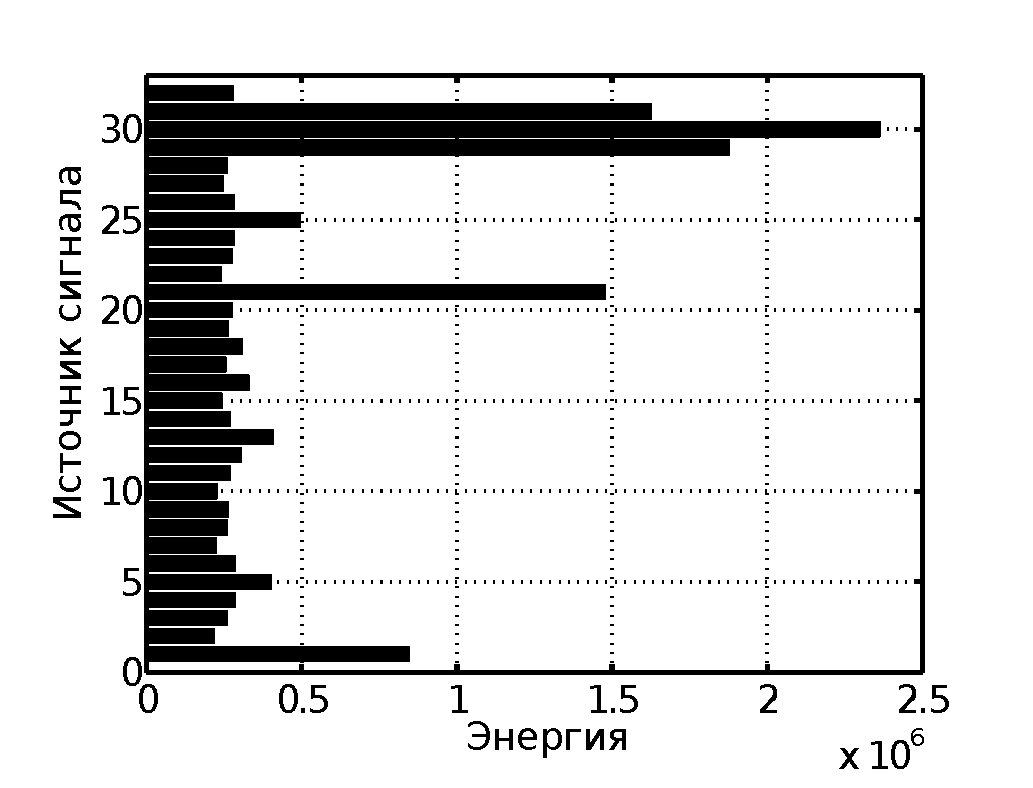
\includegraphics[width=1\linewidth]{5mhz_sats_all.eps}}
	\caption{Соотношений энергий источников сигнала}
	\label{pic:5mhz_sats_all}
\end{figure}

Рассмотрим источник сигнала 1 – рисунок \ref{pic:5mhz_sat_1}. Оценка частоты полученная параллельным коррелятором – 4.093 МГц,
оценка полученная алгоритмом на основе АР метода – 4093378.19 МГц. Видно, что система вошла в синхронизм и данные могут быть успешно демодулированы.
\begin{figure}[H]
\center\scalebox{1}{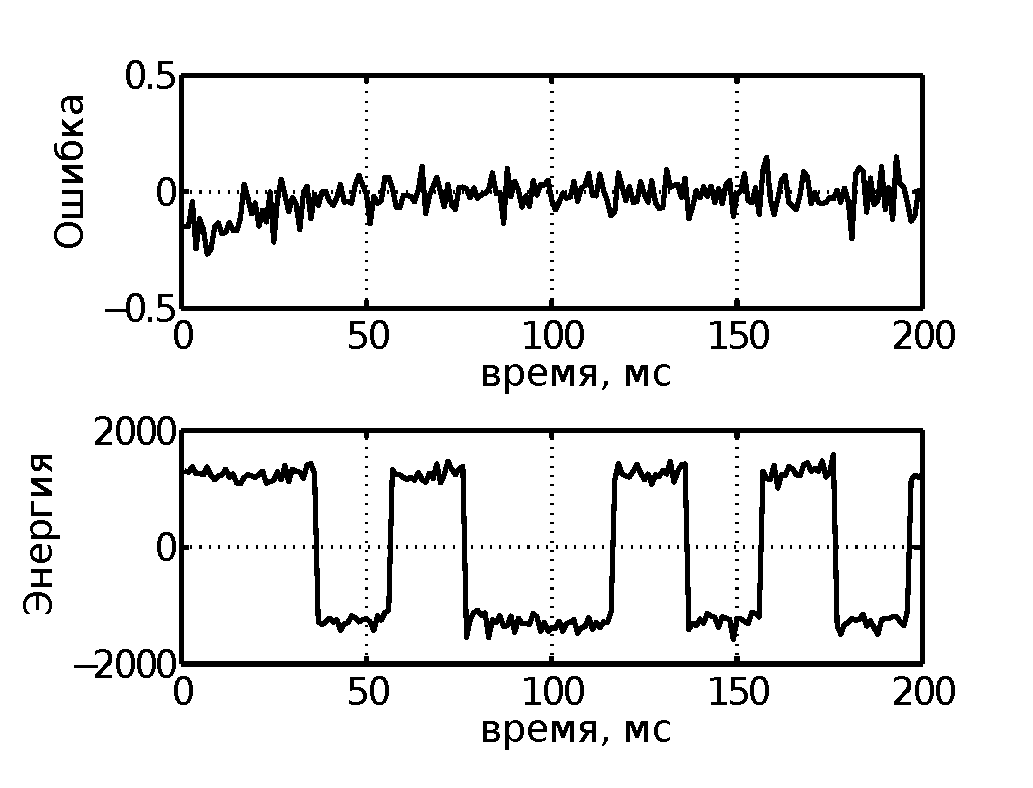
\includegraphics[width=1\linewidth]{5mhz_sat_1.eps}}
	\caption{Спутник 1}
	\label{pic:5mhz_sat_1}
\end{figure}

Рассмотрим источник сигнала 29 – рисунок \ref{pic:5mhz_sat_29}. Оценка частоты полученная параллельным коррелятором – 4.090 МГц,
оценка полученная алгоритмом на основе АР метода – 4089793.94 МГц. Видно, что система вошла в синхронизм и данные могут быть успешно демодулированы.
\begin{figure}[H]
\center\scalebox{1}{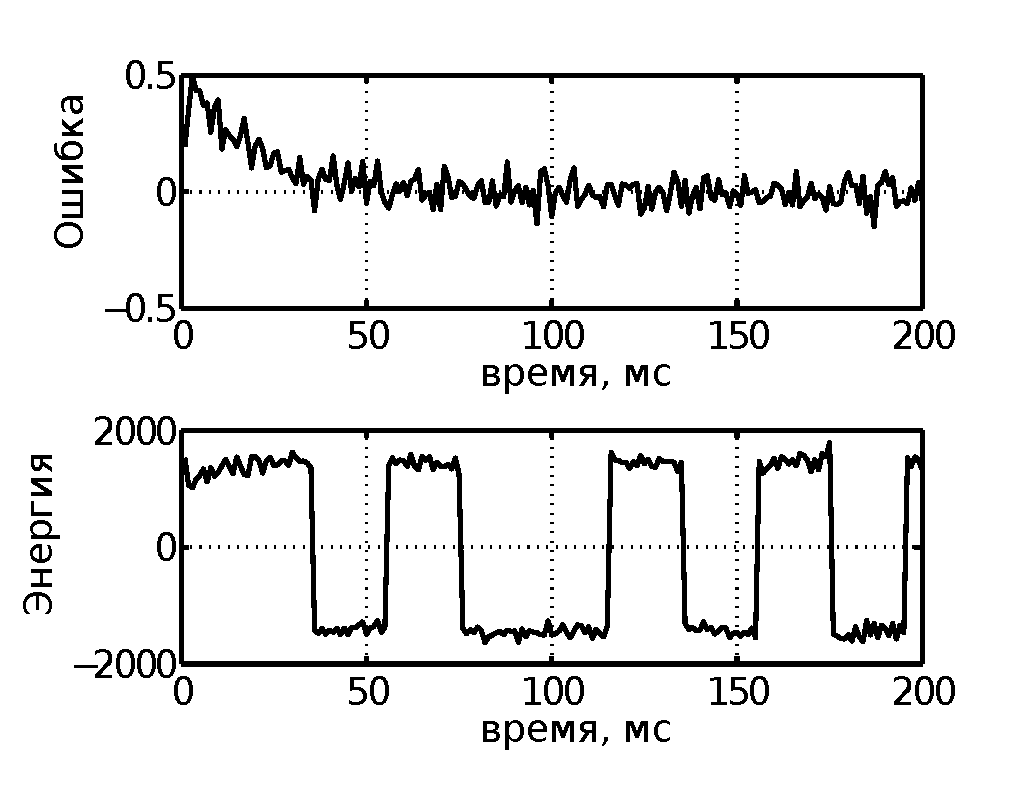
\includegraphics[width=1\linewidth]{5mhz_sat_29.eps}}
	\caption{Спутник 29}
	\label{pic:5mhz_sat_29}
\end{figure}

Рассмотрим источник сигнала 30 – рисунок \ref{pic:5mhz_sat_30}. Оценка частоты полученная параллельным коррелятором – 4.090 МГц,
оценка полученная алгоритмом на основе АР метода – 4089848.47 МГц. Видно, что система вошла в синхронизм и данные могут быть успешно демодулированы.
\begin{figure}[H]
\center\scalebox{1}{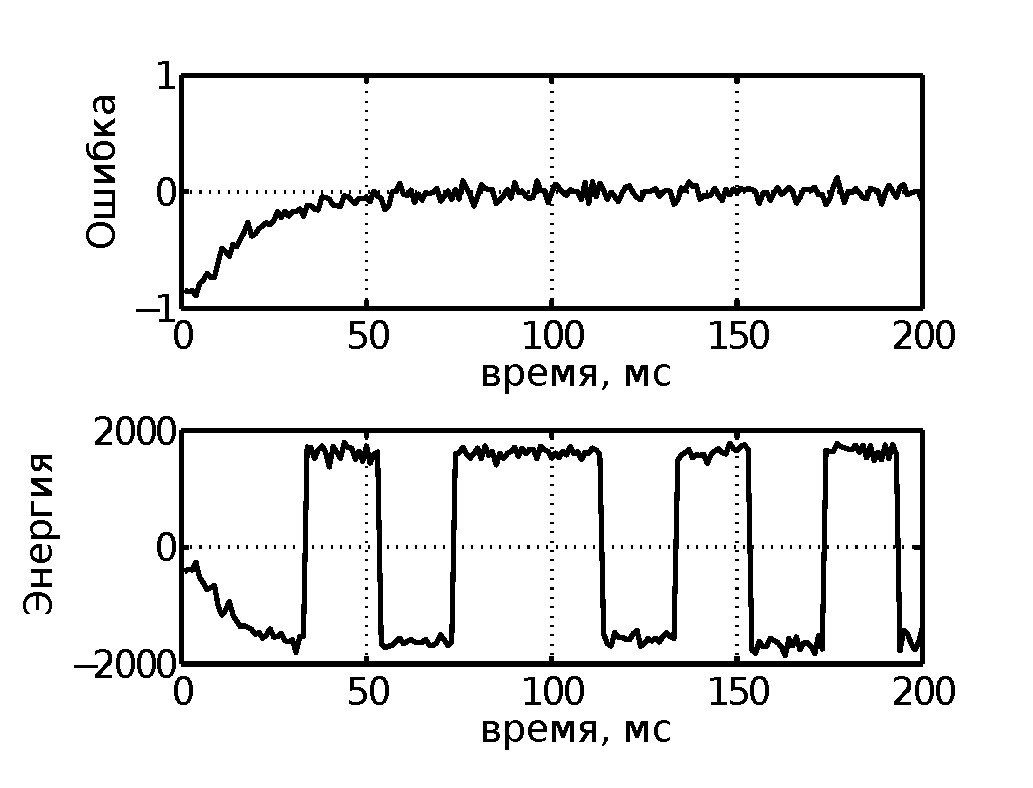
\includegraphics[width=1\linewidth]{5mhz_sat_30.eps}}
	\caption{Спутник 30}
	\label{pic:5mhz_sat_30}
\end{figure}

Рассмотрим источник сигнала 31 – рисунок \ref{pic:5mhz_sat_31}. Оценка частоты полученная параллельным коррелятором – 4.090 МГц,
оценка полученная алгоритмом на основе АР метода – 4090079.16 МГц. Видно, что система вошла в синхронизм и данные также могут быть успешно демодулированы.
\begin{figure}[H]
\center\scalebox{1}{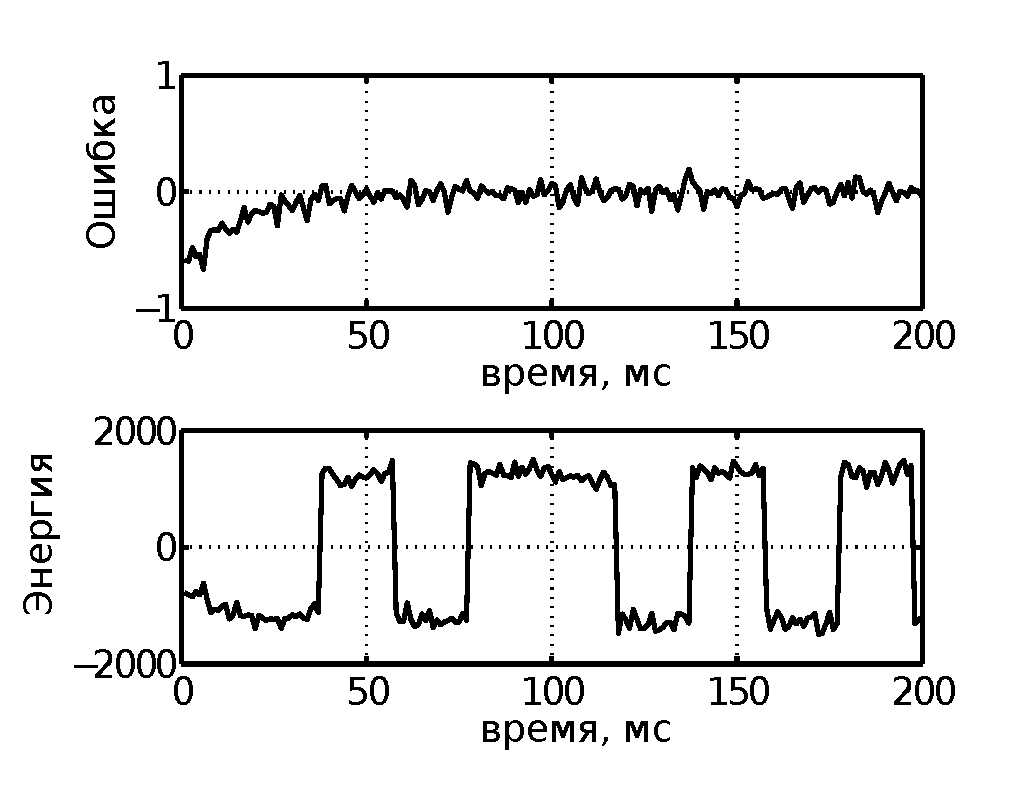
\includegraphics[width=1\linewidth]{5mhz_sat_31.eps}}
	\caption{Спутник 31}
	\label{pic:5mhz_sat_31}
\end{figure}

В то же время, параметры сигнала спутника 21, который тоже имеет достаточно высокую энергию, не смогли быть оценены - рисунок \ref{pic:5mhz_sat_21}.
\begin{figure}[H]
\center\scalebox{1}{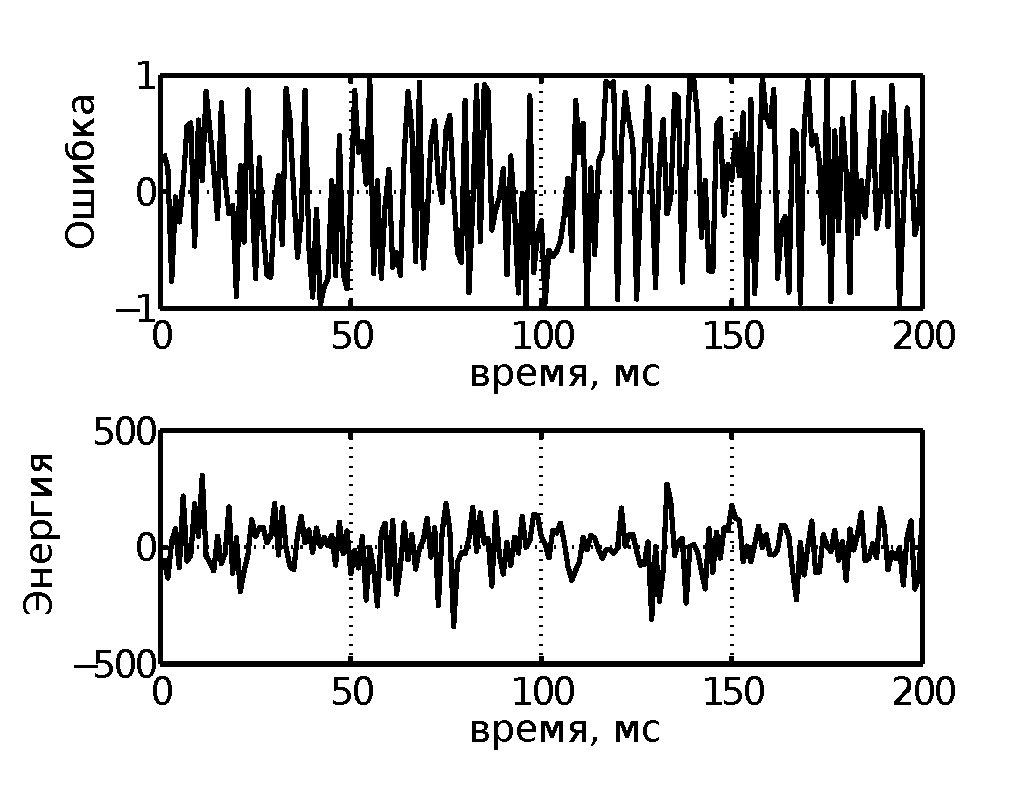
\includegraphics[width=1\linewidth]{5mhz_sat_21.eps}}
	\caption{Спутник 21}
	\label{pic:5mhz_sat_21}
\end{figure}


\section{Выводы}

\newpage
